\chapter*{Conclusion}
With the proof of the Riemann--Roch theorem in its restricted form comes the end
of this report. Discussion of the full proof of the theorem would involve some
preliminary work with sheaf theory, and unfortunately, any attempt to introduce
the necessary constructions would be either rushed or incomplete. A full
treatment of the Riemann--Roch theorem can be found in
Forster\sidenote{\footnotesize\cite{forster}}, and there are clear similarities
between this proof and the one which we have presented.

A natural next step in the study of Riemann surfaces would be to explore the
Uniformisation theorem, which is a result aimed at the classification of the
simply connected Riemann surfaces, conjectured in 1882 by Felix Klein ``in the
midst of an asthma attack''\sidenote{\footnotesize\cite{abikoff}}.

\begin{theorem}[Uniformisation Theorem]
	Every simply connected Riemann surface is biholomorphic to one of $ \mathbb{C}
	$, $ \hat{\mathbb{C}} $, or the unit disc $ \mathbb{D} $.
\end{theorem}

\begin{figure*}
	\centering
	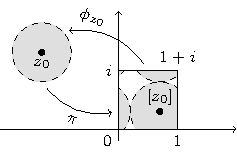
\includegraphics{uniformisation/figure}
	\caption{Drawing every simply connected Riemann surface.}
\end{figure*}

Donaldson\sidenote{\footnotesize\cite[Ch. 10]{donaldson}} explores this result
in full detail, and the proof ultimately hinges on an analogue of the main
analytic result of this report, Theorem~\ref{thm:main-thm}.

There are some further reaching consequences of the existence of meromorphic
functions which we did not explore. The most famous of these consequences was
proved by Riemann, and was the initial motivation for his pursuit of a bound on
the number of linearly independent meromorphic functions. Riemann proved that
all compact Riemann surfaces can be embedded in projective space, and hence the
study of compact Riemann surfaces can be rephrased as the study of one
dimensional projective varieties.

This duality in the theory of projective geometry and analytic manifold theory
is extended in higher dimensions, and one may consider further exploration in
the direction of closely related concepts such as Riemannian manifolds, and
further to this K\"ahler manifolds. In fact, fixing some metric on the Riemann
surface gives some element of simplification to the arguments presented in
Chapter~\ref{ch:poisson-eq}, and many of the results presented admit logical
generalisations.

% {\it
% 	It is with a heavy hand that I write the final words of this report, with
% 	tired eyes that I read it for the final time. The beauty and depth of this area
% 	of mathematics has been captivating, and I can only hope to have adequately
% 	portrayed this.
% }
